\documentclass[]{article}
\usepackage[super,numbers]{natbib}

\usepackage{fullpage}
\usepackage{listings}
\usepackage{url}
\usepackage{authblk}
\usepackage{graphicx}
\usepackage{color}
\usepackage{booktabs}

\lstset{language=Python}

% local definitions
\newcommand{\sgcomment}[1]{{\textcolor{red}{SG: #1}}}
\newcommand{\bmhcomment}[1]{{\textcolor{blue}{BMH: #1}}}
\newcommand{\aprcomment}[1]{{\textcolor{magenta}{APR: #1}}}
\newcommand{\tdwcomment}[1]{{\textcolor{cyan}{TDW: #1}}}

% cross-reference with supplement
\usepackage{xr}
\externaldocument{supplement}

\begin{document}

\title{A weakly structured stem for human origins in Africa}
\author[1]{Aaron P. Ragsdale}
\author[2]{Timothy D. Weaver}
\author[3]{Elizabeth G. Atkinson}
\author[4]{Eileen Hoal}
\author[4]{Marlo M\"{o}ller}
\author[2,6,$\dag$,*]{Brenna M. Henn}
\author[7,$\dag$,**]{Simon Gravel}
\affil[1]{Department of Integrative Biology, University of Wisconsin, Madison, WI, USA}
\affil[2]{Department of Anthropology, University of California, Davis, Davis, CA, USA}
\affil[3]{Department of Molecular and Human Genetics, Baylor College of Medicine, TX, USA}
\affil[4]{DSI-NRF Centre of Excellence for Biomedical Tuberculosis Research; South African Medical Research Council Centre for Tuberculosis Research; Division of Molecular Biology and Human Genetics, Faculty of Medicine and Health Sciences, Stellenbosch University, Cape Town, South Africa}
\affil[6]{UC Davis Genome Center, University of California, Davis, Davis, CA, USA}
\affil[7]{Department of Human Genetics, McGill University, Montreal, QC, Canada}
\affil[$\dag$]{Co-Corresponding Authors}
\affil[*]{bmhenn@ucdavis.edu}
\affil[**]{simon.gravel@mcgill.ca}
\maketitle

\abstract{
While a modern human origin within Africa is now broadly accepted, considerable
uncertainty surrounds specific models of divergence and migration across the
continent. Progress is hampered by a paucity of fossil and genomic data, as
well as variability in dating. Here we use linkage disequilibrium and
diversity-based statistics, optimized for rapid, complex demographic inference
to discriminate among such models. We infer detailed demographic models for
populations across Africa, including representatives from eastern and western
groups, as well as 44 newly whole-genome sequenced individuals from the Nama
(Khoe-San). Despite the complexity of African population history, present-day
population structure dates back to Marine Isotope Stage (MIS) 5. The earliest
population divergence among contemporary populations occurs 120-135kya, between
the Khoe-San and other groups. Prior to the divergence of contemporary African
groups, we infer long-lasting structure between two or more weakly
differentiated ancestral \emph{Homo spp.} populations connected by gene flow over
hundreds of thousands of years (i.e. a weakly structured stem). We find that
weakly structured stem models provide more likely explanations of polymorphism
that had previously been attributed to contributions from archaic hominins in
Africa.
In contrast to models with archaic introgression, we predict that fossil
remains from coexisting ancestral populations should be morphologically
similar.
Despite genetic similarity between these populations, an inferred 1--4\%
of genetic differentiation among contemporary human populations can be
attributed to genetic drift between stem populations.
We show that model misspecification explains variation in previous
divergence time estimates and argue that studying a suite of models is key to
robust inferences about deep history.
}

\section*{Introduction}

Archaeological sites from the Middle Stone Age (approx. 300kya-40kya) are widely
distributed across Africa, and are particularly well represented in the
northern, eastern and southern parts of the continent. Similarly, fossil crania
such as those from the sites of Jebel Irhoud \citep{Hublin2017-cq}, Herto
\citep{White2003-bk} and Klasies River \citep{Deacon1995-rx} demonstrate that
anatomically derived \emph{Homo sapiens} features were also present across the
continent during this period. It has been difficult to reconcile these lines of
evidence with evidence from genomics, which have suggested a predominantly
tree-like model of recent population divergence from a single ancestral
population. It is unclear whether fossil specimens and archaeological sites
represent populations which contributed to our ancestors as population
precedents, or were local “dead-ends” from which contemporary \emph{Homo
sapiens} do not descend. Recently, synthetic attempts to reconcile genetic and
paleoanthropological data include proposals for a Pan-African origin of
\emph{Homo sapiens} by which populations in many regions of the continent
contributed to the formation of Homo sapiens beginning at least 300kya
\citep{Stringer2016-mj,Scerri2018-nl,Scerri2019-xg}.

Genetic models have been hampered in their contribution to this discussion
because they primarily assume (or, at least, have been tested under) a
tree-like model of isolation-with-migration. Alternative theoretical scenarios
have been proposed, such as stepping stone models \citep{Arredondo2021-qa} or
population coalescence and fragmentation \citep{Scerri2019-xg}. These
approaches are more challenging to interpret and fit to data. However, new
population genetic tools now allow for inference involving tens to
hundreds of genomes from multiple populations and greater complexity
\citep{Kamm2020-vn,Ragsdale2019-nt,Speidel2019-nj}. Inspired by evidence for
Neanderthal admixture with modern humans in Eurasia, several recent articles
have shown that introducing an archaic ghost population contributing to African
populations in the period surrounding the Out-of-Africa migration event
substantially improves the description of genetic data relative to
single-origin models
\citep{Plagnol2006-lt,Hammer2011-bx,Hsieh2016-gk,Hey2018-pw,Ragsdale2019-nt,Durvasula2020-td,Lorente-Galdos2019-vz,Durvasula2020-td}.
This has driven speculation about the geographic range of this ghost
population, possible links to specific archaic remains, and the possibility of
finding ancient DNA evidence (e.g., \citet{Hsieh2016-gk}). However, these prior
articles share two weaknesses. First, they only contrast a single-origin model
with an archaic admixture model, leaving out other plausible models
(Figure~\ref{fig:supp-possible-models} and \citet{Henn2018-rf}). Second, they
focus on a small subset of African diversity, either because of small sample
sizes (2-5 genomes) or because they rely on 1000 Genomes data which only
recruited populations of recent West African ancestry. While ancient DNA from
Eurasia has helped us understand early human history outside of Africa, there
is no comparably ancient DNA to elucidate early history in Africa.

Here, we therefore aim to discriminate among a broader set of demographic
models by interrogating the genomes of contemporary populations. We take as our
starting point 4 classes of models (single population expansion, single
population expansion with regional persistence, archaic admixture, and
multi-regional evolution, Figure~\ref{fig:supp-possible-models}), using 290
genomes from southern, eastern, and western Africa as well as Eurasia. By
including geographically and genetically diverse populations across Africa, we
infer demographic models that explain more aspects of genetic diversity in more
populations than previously reported. These analyses confirm the inadequacy of
tree-like models and provide an opportunity to directly evaluate a wide range
of alternative models.

\section*{Results}

We inferred detailed demographic histories using 4x-8x whole-genome sequencing
data for four diverse African populations, comprising the Nama (Khoe-San from
South Africa, newly presented here), Mende (from Sierre Leone, MSL from the
Phase 3 1000 Genomes Project \citep{1000_Genomes_Project_Consortium2015-zq}),
Gumuz (recent descendents of a hunter-gatherer group from Ethiopia
\citep{Gurdasani2015-qy,Gopalan2019-wd}), and Eastern African agriculturalists
(Amhara and Oromo from Ethiopia \citep{Gurdasani2015-qy}). The Amhara and Oromo
populations, despite speaking distinct Afro-Asiatic languages, are highly
genetically similar \citep{Pagani2015-pz,Gopalan2019-wd} and thus the two
groups were combined for a larger sample size (Figure~\ref{fig:1}). We also
included the British (GBR) from the 1000 Genomes Project in our demographic
models as a representative source of back-to-Africa gene flow and recent
colonial admixture in South Africa. Finally, we used a high-coverage ancient
Neanderthal genome from Vindija Cave, Croatia \citep{Prufer2017-kk} to account
for archaic gene flow from Neanderthals in non-Africans and gauge the relative
time depth of divergence, assuming Neanderthals diverged 550kya from a common
stem. For each population, we computed low-order allele frequency and linkage
disequilibrium (LD) statistics that are well suited for both low- and
high-coverage genomes \citep{Ragsdale2019-nt,Ragsdale2020-nz}. Using a
maximum-likelihood inference framework, we then fit to these statistics a
family of parameterized demographic models that involve population splits, size
changes, continuous and variable migration rates, and punctuated admixture
events, to learn about the nature of population structure over the past million
years.

\begin{figure}[ht!]
    \centering
    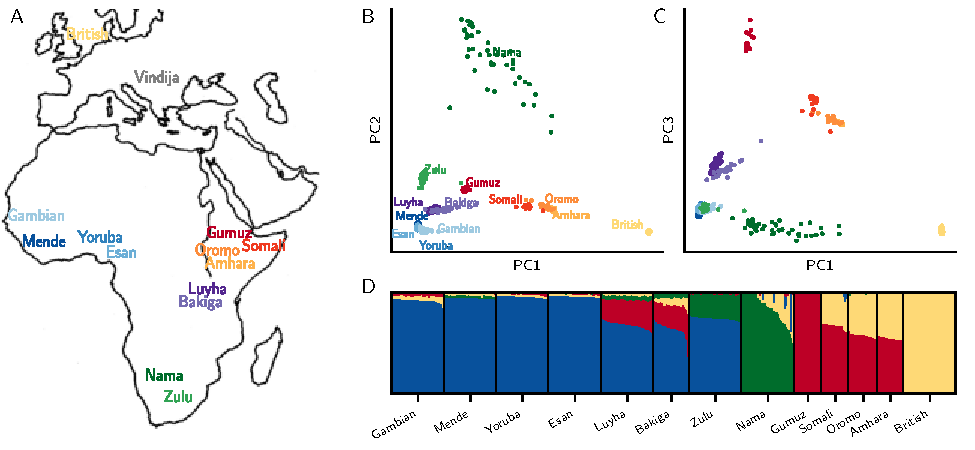
\includegraphics{figures/fig1.pdf}
    \caption{
        \textbf{Geography and genetic diversity within Africa.}
        (A) The combined 1000 Genomes and AGRP datasets include populations from
        West, East, and South Africa. Both PCA (B, C) and \texttt{ADMIXTURE}
        (D) illustrate the well-characterized high levels of genetic diversity
        and signatures of recent migration and gene flow within Africa.
        We built parameterized models using the newly-sequenced Nama from South Africa, Mende
        from Sierre Leone, Gumuz, Oromo and Amhara from Ethiopia, and the
        British and Vindija Neanderthal individual (bold fonts).
        \aprcomment{work on this caption}
    }
    \label{fig:1}
\end{figure}
   
\subsection*{A Late Middle Stone Age common ancestry for contemporary humans}

We began with a model of geographic expansion from a single ancestral,
unstructured source followed by migration between populations, without allowing
for contribution from an archaic African lineage or population structure prior
to the expansion (Figure~\ref{fig:supp-possible-models}A). As expected
\citep{Ragsdale2019-nt}, this first model was a poor fit to the data
qualitatively (Figure~\ref{fig:supp-single-origin-fits}) and quantitatively
(log-likelihood ($LL$) $\approx -189,400$, Table~\ref{tab:supp-single-origin}).
We next explored a suite of models in which population structure predates the
differentiation of contemporary groups, including models allowing for ancestral
reticulation (Figure~\ref{fig:supp-possible-models}B), archaic admixture
(Figure~\ref{fig:supp-possible-models}C), and African multi-regionalism
(Figure~\ref{fig:supp-possible-models}D).

Regardless of the model choice for early epochs, inference of human demographic
history for the last 150kya was remarkably robust. The earliest divergence among
contemporary human populations differentiates the southern African Nama from
other African groups between 110--135kya, with low to moderate levels of
subsequent gene flow (Table \ref{tab:migration-rates}). In none of the
high-likelihood models which we explored did the divergence between Nama and
other populations exceed $\sim$140kya. 
We conclude that geographic patterns of contemporary \emph{Homo sapiens} population structure
date back to the late Middle Stone Age in Africa, likely arising during MIS 5.
Although we find evidence for earlier population structure in Africa (see
below), present-day populations cannot be easily mapped onto these more ancient
stem groups as only a small proportion of drift between modern populations can
be attributed to drift between stems (Figures~\ref{fig:3} and
\ref{fig:supp-f4s-single-origin}--\ref{fig:supp-f4s-merger-with-stem-migration}). 

Given this consistency in inferred recent history and the numerical challenge
of optimizing a large number of parameters, we fixed several parameters related
to recent population history so as to focus on more ancient events (see below). Fixed parameters included
divergence time the time of divergence between Western and Eastern African populations,
set to 60kya, just prior to the split of Eurasians and East Africans set to 50kya. 
We also fixed the amount of admixture from Neanderthals to Europeans directly
following the out-of-Africa migration which was set to 1.5\% at 45kya (Supp. Methods). Such constraints, informed by prior research,
allowed us to infer robust migration rates. For example all models infer relatively high gene flow between Eastern and Western Africa
($m\approx2\times10^{-4}$). We further find that Back-to-Africa gene flow at the beginning of the Holocene primarily
affected the ancestors of the Ethiopian agricultural populations, comprising
over half of their genetic ancestry, estimated to be 64--65\%. The past 5,000
years also saw major demographic changes, including strong population growth
for Western Africans as they specialized in yam and oil palm agriculture
(estimated 3-fold growth). We observe significant gene flow from the Amhara and
Oromo into the Nama, a signal which is likely a proxy for the movement of
Eastern African caprid and cattle pastoralists
\citep{Henn2008-xo,Breton2014-xb}, here estimated to constitute a 25\% ancestry
contribution 2,000 ya. Colonial period admixture from Europeans into the Nama
was estimated at 15\%, similar to proportions inferred by \texttt{ADMIXTURE}
\citep{Alexander2009-sw} (Figure~\ref{fig:1}).

\begin{figure}[t!]
    \centering
    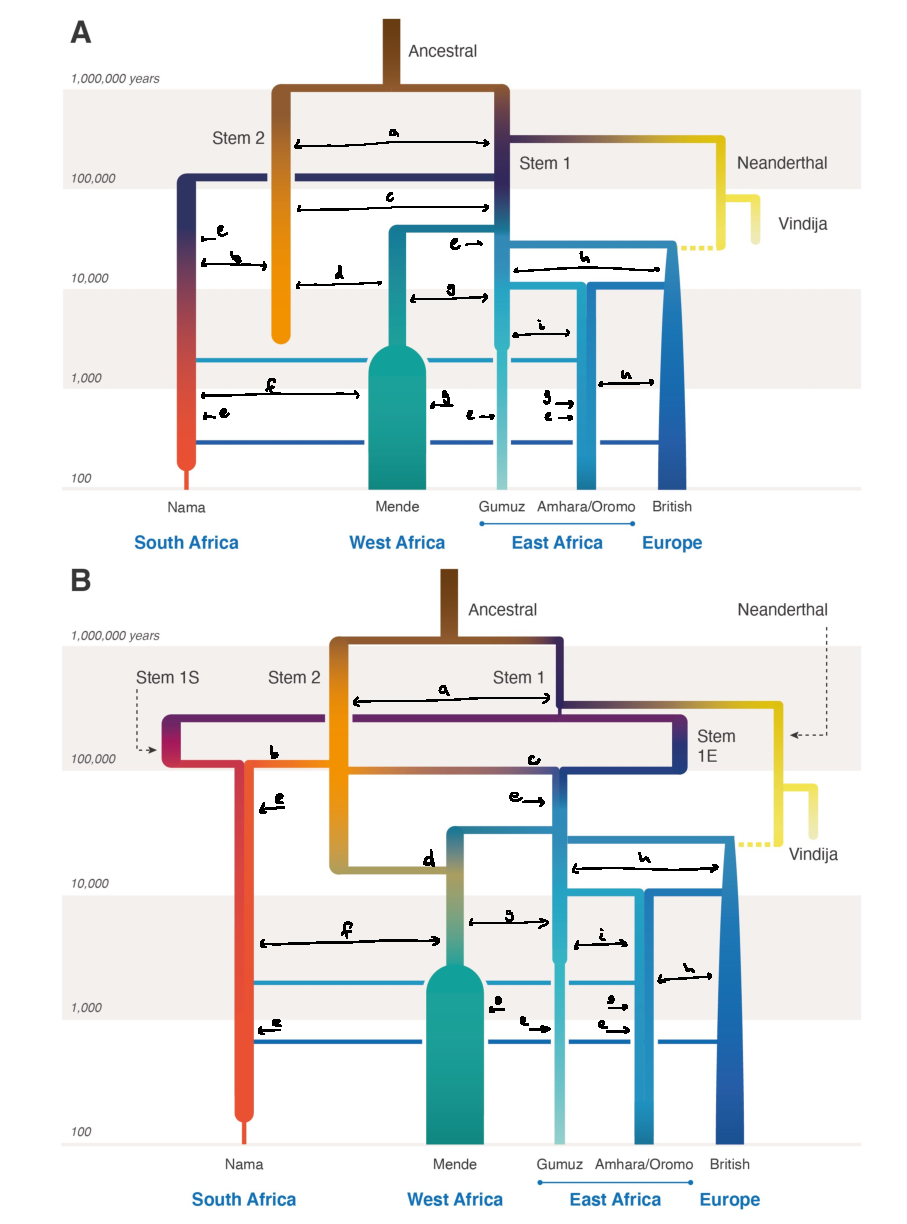
\includegraphics[width=0.5\textwidth]{figures/fig2}
    \caption{
        \textbf{Two best fit models with a weakly structured stem.}
        In both the the parameterizations of early population structure,
        continuous migration (A) and multiple mergers (B), models
        that include ongoing migration between stem populations outperform
        those in which stem populations are isolated. Most recent populations are
        connected by continuous, reciprocal migration that are incidated by 
        double-headed arrows (labels matched to migration rates and divergence
        times in Table~\ref{tab:migration-rates}), and which lasts for the
        duration of concurrence of contemporaneous populations. The
        merger-with-stem-migration model (B) outperformed the
        continuous-migration model (A), $LL=-102,600$ vs $-115,500$,
        respectively.
    }
    \label{fig:2}
\end{figure}

\begin{table}[t!]
    \centering
    \scriptsize
    \begin{tabular}{lllrrrr}
        \toprule
        \textbf{Likelihood} & \textbf{Label} & \textbf{Population Pair} &
            \textbf{Divergence} & \textbf{Migration rate} & \textbf{Migration} \\
        & & & 
            \textbf{Time (kya)} & \textbf{per generation} & \textbf{duration (ky)} \\
        \midrule
        \textbf{Continuous Model} & & & & & \\
        LL= -115,500 & a & Stem 1, Stem 2 & 1,163 & 6.43e-5 & 1,028 \\
        & b & Stem 2, Nama & NA & 5.82e-5 & 130 \\
        & c, d & Stem 2, Other Africans* & NA & 3.10e-5, \textbf{1.64e-4} & 130, 55 \\
        & e, f & Nama, Other Africans* & 135 & 4.1e-5, 9.8e-6 & 135, 60 \\
        & g & Mende, East Africans & 60 & \textbf{2.14e-4} & 60 \\
        & h & East Africans, British & 50 & 4.17e-5 & 50 \\
        & i & Gumuz, Amhara/Oromo & 12 &\textbf{3.36e-4} & 12 \\
        \textbf{Merger Model} & & & & & \\
        LL= -102,600 & a & Stem 1, Stem 2 & 1,442 & \textbf{1.16e-4} & 963 \\
        & -- & Stem 1S, Stem 1E & 479 & 0 (fixed) & -- \\
        & b & Stem 2 to Nama & 119 & \textbf{0.71} & pulse \\
        & c & Stem 2 to Stem 1E & 98 & \textbf{0.50} & pulse \\
        & d & Stem 2 to Mende & 25 & \textbf{0.18} & pulse \\
        & e, f & Nama, Other Africans* & 119 & 4.4e-5, 7.1e-6 & 119, 60 \\
        & g & Mende, East Africans* & 60 & \textbf{1.98e-4} & 60 \\
        & h & East Africans, British & 50 & 3.87e-5 & 50 \\
        & i & Gumuz, Amhara/Oromo &12 & \textbf{3.59e-4} & 12 \\
        \bottomrule
    \end{tabular}
    \caption{
        \textbf{Migration and divergence parameters from best fit models.}
        Labeled migration rates correspond to symmetric continuous migration
        bands shown in Figure~\ref{fig:2}. Both the continuous migration and
        merger models inferred a relatively deep split of human stem branches,
        though they were connected by ongoing migration that maintained their
        genetic similarity.
        *: The ancestors of the Nama diverged from other African groups
        $\sim$120--135kya, which later branch into West and East African
        groups 60kya. Migration rates and durations are shown for 1) East Africans
        and their ancestors, and 2) the Mende, respectively.
    }
    \label{tab:migration-rates}
\end{table}

\subsection*{Deep but connected population structure within Africa}

To account for population structure prior to 135kya, three of our four models allowed for two or more
“stem” populations which could diverge either before or after the Neanderthal
split. We considered models both with and without migration between these stem
populations, and in both cases we tested two different types of gene exchange
during the expansion phase. 1) One of the stem population expands (splits into
contemporary populations), and the other stem population(s) has continuous
symmetric migration with those populations; or 2) one or more of the stem
populations expands, with instantaneous pulse (or “merger”) events from the
other stem population, so that recent populations are formed by mergers of multiple ancestral populations. Depending on parameter values,
this scenario encompasses archaic introgression and
fragmentation-and-coalescence models. For many parameters, confidence intervals based on bootstrapping are relatively narrow
(Tables~\ref{tab:supp-single-origin}--\ref{tab:supp-merger-with-stem-migration}),
reflecting an informative statistical approach. Model assumptions
have, however, a larger impact on parameter estimates (and thus, uncertainty). To convey model uncertainty, we
highlight features of the two inferred models with high likelihoods. These are referred to as the
“multiple-merger” and the the “continuous-migration” model. Both allow for
migration between stem branches, but differ primarily in the timing of the
early divergence of stem populations and their relative $N_e$
(Figure~\ref{fig:2}). The two models also differ in the mode of divergence
during the Middle Stone Age.

Allowing for continuous migration between the stem populations substantially
improved the fits relative to zero migration ($LL \approx -102,600$ vs.
$-107,700$ in the merger model and $LL \approx -115,500$ vs. $-126,600$ with
continuous migration). With continuous migration between stems, population
structure extends back to 1.1--1.4Mya (Table~\ref{tab:migration-rates}).
Migration between the stems in these models is moderate, with a fraction of
migrant lineages each generation estimated as
$m=6.43\times10^{-5}-1.16\times10^{-4}$. For comparison, this is similar
to inferred migration rates between connected contemporary populations over the
past 50kya (Table~\ref{tab:migration-rates}). This ongoing (or at least,
periodic) gene flow qualitatively distinguishes these models from previously
proposed archaic admixture models (Figure~\ref{fig:supp-possible-models}C) as
the early branches remain closely related (Figure 3). 
 
Under the continuous-migration model, one of the two stems diverges into
lineages leading to contemporary populations in western, southern and eastern
Africa, and the other (Stem 2) contributes variable ancestry to those
populations. This migration from Stem 2 is highest with the Mende
($m=1.6\times10^{-4}$) compared to the Nama and East African populations
($m=5.8\times10^{-5}$ and $3.1\times10^{-5}$, respectively), with migration
allowed to occur until 5kya. A
sampled lineage from the Nama, Mende, and Gumuz have probabilities of being in
Stem 2 at the time of Stem 1 expansion (135ka) of approximately $0.145$, $0.2$,
and $0.13$, respectively, though these probabilities change over time,
precluding the notion of a fixed admixture proportion.

In contrast, under the multiple-merger model, stem populations merge with
varying proportions to form the different contemporary groups. 
We observe a sharp bottleneck in Stem 1 down to $N_e=117$ after the split of
the Neanderthal branch. This represents the lower bound allowed in our
optimization (i.e. 1\% of the ancestral $N_e$), although the size of this
bottleneck is poorly constrained ($\sigma_{N_e}=838$). After a long period of
exchange with Stem 2, Stem 1 then fractures into “Stem 1E” and “Stem 1S”
479kya. The timing of this divergence was also poorly constrained ($\sigma_T=
166$kya). These populations evolve independently until approximately 119kya
when Stem 1S and Stem 2 combine to form the ancestors of the Nama, with
proportions 29\%, 71\% respectively. Similarly, Stem 1E and Stem 2 combine in
equal proportions (50\% each) to form the ancestors of the Western Africans and
Eastern Africans (and thus also all individuals who later disperse during the
Out of Africa event). Finally, the Mende receive a large additional pulse of
gene flow from Stem 2, replacing 18\% of their population 25kya. The later Stem
2 contribution to the Western African Mende resulted in better model fits (LL).
This may indicate that an ancestral Stem 2 population occupied Western or
Central Africa, broadly speaking. The differing proportions in the Nama and
Eastern Africans may also indicate geographic separation of Stem 1S in southern
Africa and Stem 1E in eastern Africa. 

\begin{figure}[t!]
    \centering
    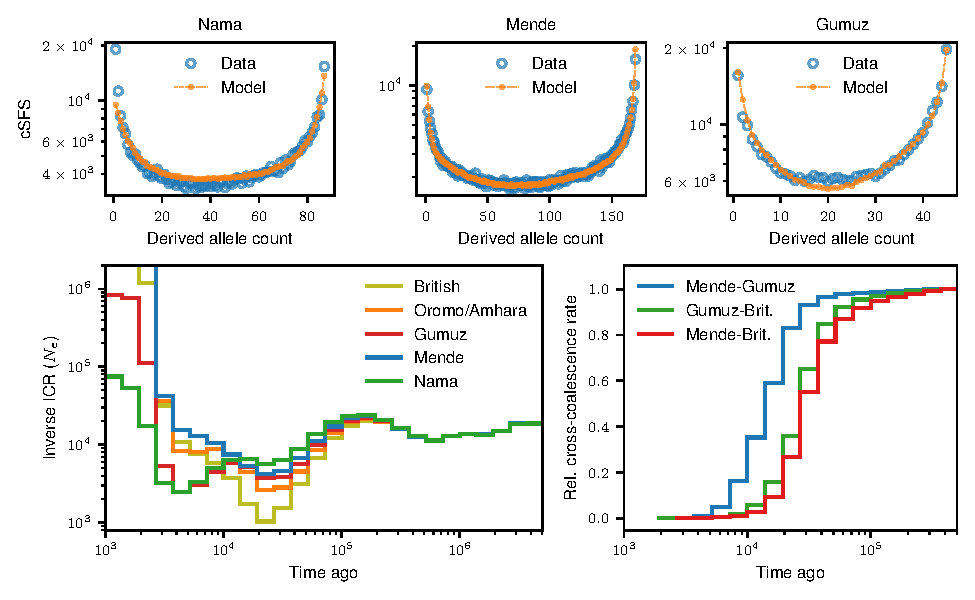
\includegraphics{figures/fig3.pdf}
    \caption{
        \textbf{Predicted population structure over time.}
        From the best fit models of our two parameterizations (top row:
        continuous migration, bottom row: merger with stem migration), we computed
        predicted differentiation between contemporaneous populations over time
        as $H_{i,j}$, the expected pairwise diversity between two samples, one
        each from populations $i$ and $j$.
        We also computed the proportion of drift between pairs of sampled
        populations that aligns with drift between populations in the past
        ($\alpha^2$, see Section~\ref{sec:f4} in the Supplement).
        While both models inferred population structure to extend deep into the
        past, the ancient structure contributes relatively little to present-day
        differentiation between human populations.
    }
    \label{fig:3}
\end{figure}

\subsection*{Reconciling multiple lines of genetic evidence}

Previous studies have found support for archaic admixture in Africa using
two-locus statistics \citep{Hsieh2016-gk,Ragsdale2019-nt}, the conditional SFS
(cSFS) \citep{Durvasula2020-td}, and reconstruction of gene genealogies
\citep{Speidel2019-nj}. However, none of these studies considered a weakly
structured stem. We validated our inferred models with additional independent
approaches. We find that the observed cSFS (conditioned on the derived allele
being carried in the Neanderthal sample) is very well-described by the merger
model (Figures~\ref{fig:4}A-C and
\ref{fig:supp-csfs-single-origin}--\ref{fig:supp-csfs-merger-with-stem-migration}),
even though this statistic was not used in the fit. Both models outperform
archaic models fit directly to the cSFS (for example, compare with Figure~1 in
\citet{Durvasula2020-td}).

\begin{figure}[t!]
    \centering
    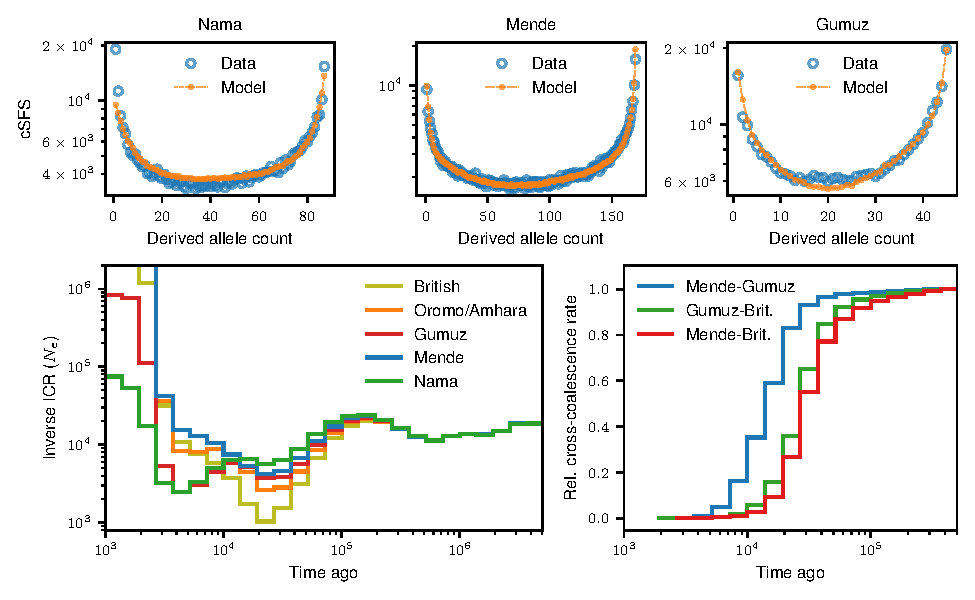
\includegraphics{figures/fig4}
    \caption{
        \textbf{Model validation using independent statistics.} (A--C) Using
        our best fit models to the LD and pairwise diversity statistics, we
        simulated expected conditional site-frequency-spectra (cSFS) and
        compared to the observed cSFS from the data. Our inferred models
        provide a good fit to the data, even though these were not used in our
        inference. Across the three populations, ancestral state
        misidentification was consistently inferred to be 1.5--1.7\% for
        intergenic loci (Supp. Methods). (D, E) We used Relate
        \citep{Speidel2019-nj} to reconstruct genome-wide gene genealogies,
        which we used to estimate coalescence rate trajectories and
        and cross-coalescence rates between pairs of populations. While
        coalescence rate distributions are informative statistics about past
        evolutionary processes, interpretation can be hindered by migration and
        population structure, and translating relative cross-coalescence rate
        curves (RCCR) into population divergence times is especially prone
        to misinterpretation. For example, the Mende-Gumuz comparison shows
        a more recent increased RCCR than either population with the British,
        a pattern that is recapitulated under our best-fit model, even though
        the Mende-Gumuz split occurs prior to the Gumuz-British split.
    }
    \label{fig:4}
\end{figure}

We used \texttt{Relate} \citep{Speidel2019-nj} to infer the distribution of
coalescence rates over time, which are commonly interpreted as effective
population size histories. Trajectories of $N_e$ from prior studies strongly
support a bottleneck in Out of Africa populations. African populations also dip
in effective size around 100-200kya, although this decrease is more modest than
the OOA event \citep{Mallick2016-lx}. One possible explanation is that
ancestral population structure during the Middle Stone Age inflated $N_e$ and
subsequent gene flow among ancestral Africans resulted in a more recent
decreased $N_e$ \citep{Mazet2016-wn}.
%To our knowledge, explicit comparisons of this hypothesis with SMC-style
%approaches have not been published.
We simulated genomic data under four inferred demographic models to compare
with observed coalescence rate histories. All models, including the
single-origin model, generate multi-modal curves indicating that the ancestral
increase in $N_e$ between 100kya-1Mya is a general feature of the coalescent
rate in humans, although none of the models perfectly match the exact timing of
the early fluctuations in $N_e$ observed in the data.
%Simulated Relate Ne curves under the CM and MM are distinguished by having 2
%and 3 modes, respectively.  The Continuous Migration model had the better
%qualitative fit with the data, but the ancestral mode was shifted further back
%in time relative to the data.
Each simulated model also underestimated the level of population growth during
the Holocene, indicating additional free parameters are necessary to refine
these growth rates.

Relative cross-coalescence rates (rCCR) have recently been used to estimate
divergence between a pair of populations, as measured by the rate of
coalescence between two groups divided by the mean within population
coalescence. Simulations of rCCR accuracy, however, focus on a ‘clean split’
between populations whereby groups diverge without subsequent gene flow.
Published estimates of the earliest human divergences with rCCR, which range
from 150kya-100kya \citep{Bergstrom2021-iw}, may be significantly biased when
compared to more complex models with gene flow as inferred here. We find that
midpoint estimates of rCCR are poor estimates for population divergence, often
underestimating divergence time by 50\% or greater (e.g., Mende vs. Gumuz
$\sim$15kya compared to a true divergence of 60kya), and recent migration can
lead to the misordering of divergence events (Figure~\ref{fig:4}E). We suggest
that rCCR analyses which do not fit multiple parameters including gene flow
should be interpreted with caution.

\section*{Discussion}

Any attempt at building detailed models of human history is subject to model
misspecification. This is true of earlier studies, which often assumed that
data inconsistent with a single origin model must be explained by archaic
admixture. This is also true of this study. While it remains prohibitive to
fully explore the space of plausible models of early human population structure,
we sought to capture model uncertainty by exploring multiple parameterizations of
early history.
\bmhcomment{we use this phrase a lot. human or hominin? Tim?}
The best-fit models presented here include reticulation and migration between
early human populations rather than archaic admixture from long-isolated branches.
We cannot rule out that more complex models involving
additional stems, or hybrid models including both weak structure and archaic
admixture may better explain the data. Because parameters related to the split
time, migration rates, and relative sizes of the early stems were variable
across models, reflecting a degree of confounding among these parameters, we
refrained from introducing additional branches associated with more
parameters during that period.
\sgcomment{Some statement about hitting the boundary}
Rather than interpreting the two stems as representing well-defined
and stable populations over hundreds of thousands of years, we interpret the
weakly structured stem as consistent with a population coalescence and
fragmentation model \citep{Scerri2019-xg}.
Models including additional diversity within Africa,
and ancient DNA samples from Africa, could further distinguish
the archaic admixture model from the weakly-structured-stem model.

\subsection*{The Middle Stone Age in Africa}

By contrast, our inferred models paint a more consistent picture of the late
Middle Stone Age as a critical period of change, assuming that estimates from
the recombination clock accurately relate to geological chronologies
(Supporting Information).
During the Middle Stone Age, the Multiple Merger indicates three
major stem lineages in Africa, tentatively assigned to southern (Stem 1S),
eastern (Stem 1E) and western/central Africa (Stem 2). While the length of
isolation among the stems is variable across model fits, models with a period of 
divergence, isolation and then a merger event (i.e. a “reticulation”)
out-performed models with bifurcating divergence and continuous gene flow. 

A population reticulation involves multiple stems contributing genetically to
the formation of a group. One way in which this can happen is through the
geographic expansion of one or both stems. For example, if during MIS 5, either
Stem 1S from southern Africa moved northward thereby encountering the Stem 2,
or Stem 2 moved from central/western Africa southward into Stem 1S -- then we
could observe disproportionate ancestry contributions from different stems in
modern groups. We observed two merger events. The first, between Stem 1S and
Stem 2, results in the formation of an ancestral Khoe-San population ~120kya.
The second ~100kya between Stem 1E and Stem 2, results in the formation of the
ancestors of East/West Africans as well as later “Out of Africans”. The rapid
rise in sea levels and increased precipitation during MIS 5e, following a
glacial period of aridity across Africa \citep{Blome2012-lw}, might have
triggered migration inland away from the coasts, as has been suggested for the
Paleo-Agulhas plain \citep{Marean2014-pg}. 

Following these merger events, the stems subsequently fracture into
subpopulations which then appear to persist over the past ~120kya. These
subpopulations can be linked to modern-day groups despite subsequent gene flow
across the continent; for example, a genetic lineage sampled in the Nama has an
XX probability of being in the ancestral ‘southern’ subpopulation 50kya versus
XX probability of being in the ‘eastern’ subpopulation (Figure XX). We also
find that Stem 2 continued to contribute to western Africans during the Last
Glacial Period, indicative that this gene flow likely occurred in
western/central Africa (Table 1). 

\subsection*{Contrasting archaic admixture and a weakly structured stem}

Evidence for archaic admixture in Eurasia has bolstered the plausibility of
archaic admixture having also occurred in Africa. For this reason, previous
work has focused on archaic admixture to explain patterns of polymorphism
inconsistent with a single origin model. Here, we have shown that
weakly-structured-stem models better capture these patterns.
They also help explain an
ecological riddle posed by the archaic admixture model. Neanderthal populations
were separated from early \emph{Homo sapiens} by thousands of kilometers and
continental geographic barriers. By contrast, an archaic hominin population in
Africa would need to have stayed in relative reproductive isolation from the
ancestral human lineage over hundreds of thousands of years despite closer geographic
proximity and reproductive compatibility. The weakly-structured-stem model
resolves this ecological riddle by accommodating continuous or recurrent
contact between two or more groups present in Africa.

There is evidence for both deleterious and adaptive archaic-derived alleles in
modern genomes in the form of a depletion of Neanderthal ancestry in regulatory
regions \citep{Petr2019-xo} or an increased frequency of archaic-related
haplotypes such as at \emph{EPAS1} among Tibetans (e.g.,
\citet{Zhang2021-xx}). Under previous
archaic African admixture models, the estimated 8--10\% introgression rate is
much higher than Neanderthal gene flow, and would have plausibly been fertile
ground for dramatic selection for or against archaic-derived haplotypes\citep{Wall2019-ao}. By contrast, adaptation under a weakly
structured stem would have occurred continuously over much longer periods.
Patterns of polymorphism that are inconsistent with the single-stem model
predictions have been used to infer putative archaic admixed segments
\citep{Plagnol2006-lt,Hsieh2016-gk,Wall2019-ao,Durvasula2020-td}, negative
selection against such segments \citep{Wall2019-ao}, and pervasive positive
selection \citep{Schrider2017-kl}. However, such approaches are subject to high
false positives in the presence of population structure with migration
\citep{Petr2019-xo}, and their interpretation should be re-examined in light of
a weakly-structured-stem model within Africa.

Multiple studies have shown a correspondence between phenotypic
differentiation, usually assessed with measurements of the cranium, and genetic
differentiation among human populations and between humans and Neanderthals
\citep{Relethford1994-mh,Weaver2008-ho,Von_Cramon-Taubadel2009-zb}. If we
assume that this correspondence also holds for early human ancestral
populations in Africa, the weakly-structured-stem model would predict that the
fossils deriving from each of the two stems should be morphologically quite
similar (supplementary text X)\aprcomment{Will we still include this?}, even if
they are from different parts of Africa, with differences across stems closer
to those across contemporary human populations than to human-Neanderthal
differences. Differences within stems would be comparable to differences within
recent human populations. Identifying the morphological signature of ancient
structure in the fossil record will require careful analysis of many broadly
similar remains. Our model further predicts that morphologically distinct
crania such as XX and YY are unlikely representatives of branches that
contributed appreciably to modern human ancestries.

\section*{Methods}

Methods are detailed in the Supporting Information.

\section*{Acknowledgements}

We are grateful for the DNA contribution from each participant which enabled
this study; in particular we wish to highlight the generous participation of
the Richtersveld Nama community in South Africa and help from local research
assistants Willem DeKlerk and Hendrik Kaimann. Additional assistance and
community engagement was conducted by Justin Myrick, Chris Gignoux, Caitlen
Uren and Cedric Werely. We thank the African Genome Diversity Project for data
generation, including Tommy Carensten, Deepti Gurdasani, and Manj Sandhu. We
thank Sriram Sankararaman for helpful discussion. This research was
supported by an NIH grant R35GM133531 (to BMH) and XXX. The content is solely
the responsibility of the authors and does not necessarily represent the
official views of the National Institutes of Health.

\bibliographystyle{unsrtnat}
\bibliography{paper}
\end{document}
